\section{Regular languages}
\label{sec:regular}

Regular languages can be described in three ways that turn out to be
equivalent: regular grammars generate them, regular expressions describe them
and finite automata recognize them. This section follows Hopcroft, Motwani and
Ullman~\cite[Ch.~3--4]{hopcroft2007automata}.

\subsection{Regular grammars}

\begin{definition}
A \textbf{regular grammar} (type 3) is a context-free grammar whose rules have
one of two restricted forms. In a \textbf{right regular grammar} every rule is
$A ::= a$ or $A ::= aB$; in a \textbf{left regular grammar} every rule is
$A ::= a$ or $A ::= Ba$, with $A, B \in N$ and $a \in \Sigma$.
\end{definition}

At most one nonterminal appears on the right side of a rule, always at the
same end. That restriction is what makes the languages regular.

\paragraph{A right grammar.} The lecture uses
$\mathcal{G}_{3r} = \langle \{A, B\}, \{a, b\}, A, P_{3r} \rangle$ with the rules
\[
A ::= a \qquad A ::= aB \qquad A ::= bA \qquad A ::= b \qquad B ::= bB \qquad B ::= a.
\]
Grouping the rules of each nonterminal with \texttt{|} gives a shorter
version,
\begin{lstlisting}
A ::= a | aB | bA | b
B ::= bB | a
\end{lstlisting}
and with EBNF the recursion can be replaced by repetition: \texttt{bA} means
any number of $b$'s before the rest, and \texttt{bB} any number of $b$'s
before the final $a$.
\begin{lstlisting}
A ::= b* (a | b | a B)
B ::= b* a
\end{lstlisting}
This last form is less common, but it shows the language directly: some
$b$'s, then $a$, or $b$, or an $a$ followed by some $b$'s and an $a$. As a
regular expression, $b^*(a \mid b \mid ab^*a)$.

The word $bbbabba$ is generated by a derivation in which every step adds one
terminal at the left of the single nonterminal:
\[
A \Rightarrow bA \Rightarrow bbA \Rightarrow bbbA \Rightarrow bbbaB \Rightarrow bbbabB
  \Rightarrow bbbabbB \Rightarrow bbbabba.
\]
The lecture notes that this grammar defines a common data structure: a word
of a right grammar is built one symbol at a time from the left, like a list.

\paragraph{A left grammar.} The second example is
$\mathcal{G}_{3l} = \langle \{S, A\}, \{a, b\}, S, P_{3l} \rangle$ with
\[
S ::= Abbb \qquad S ::= Sb \qquad A ::= Aa \qquad A ::= aa.
\]
The rules build the word from the right: $S$ adds $b$'s at the end and $A$
adds $a$'s at the end of the $a$ part. The shortest word is
$S \Rightarrow Abbb \Rightarrow aabbb$, and the language is $aaa^*bbbb^*$: at least two
$a$'s followed by at least three $b$'s.

\paragraph{Parse trees.} A parse tree represents the structure of a word
according to the production rules; the children of a node are the symbols of
the right side of the rule applied. Figure~\ref{fig:regular-trees} shows the
trees of the two derivations above. A right grammar produces a tree that grows
down to the right, a left grammar one that grows down to the left.

\begin{figure}[h]
\centering
\begin{forest}
  for tree={font=\small, s sep=4mm, l sep=3mm},
  [A [b] [A [b] [A [b] [A [a] [B [b] [B [b] [B [a]]]]]]]]
\end{forest}
\hspace{2cm}
\begin{forest}
  for tree={font=\small, s sep=4mm, l sep=3mm},
  [S [A [a] [a]] [b] [b] [b]]
\end{forest}
\hspace{1cm}
\begin{forest}
  for tree={font=\small, s sep=4mm, l sep=3mm},
  [S [S [A [A [a] [a]] [a]] [b] [b] [b]] [b]]
\end{forest}
\caption{Parse trees for $bbbabba$ in $\mathcal{G}_{3r}$ (left), and for $aabbb$
and $aaabbbb$ in $\mathcal{G}_{3l}$ (right).}
\label{fig:regular-trees}
\end{figure}

Both grammars can be written in Rascal directly. They are \texttt{lexical}
because no spaces may appear between the symbols:
\codelines{Rascal}{rascal/src/Regular.rsc}{8}{9}
\codelines{Rascal}{rascal/src/Regular.rsc}{11}{12}
The tests compare each grammar with its regular expression on every word over
$\{a,b\}$ of length up to 8.

\paragraph{From grammars to languages.} The language of a grammar is the set of
words of terminals that can be derived from the initial symbol,
\[
L(\mathcal{G}) = \{ \omega \in \Sigma^* \mid S_0 \Rightarrow^* \omega \},
\]
where $\Rightarrow^*$ is a sequence of applications of the rules in $P$.

\subsection{Regular expressions}

\begin{definition}
The \textbf{regular expressions} over $\Sigma$ are defined inductively:
\begin{itemize}
  \item $\lambda$ is a regular expression (the empty word);
  \item every $\sigma \in \Sigma$ is a regular expression;
  \item if $\alpha$ and $\beta$ are regular expressions, so are $\alpha \mid \beta$
    (union, or option), $\alpha\beta$ (concatenation) and $\alpha^*$ (Kleene star,
    zero or more repetitions).
\end{itemize}
Two abbreviations are common: $\alpha^+ = \alpha\alpha^*$ (one or more) and
$\alpha? = \alpha \mid \lambda$ (optional, also written $[\alpha]$).
\end{definition}

Regular expressions are a declarative way to describe the words of a regular
language. They are used to recognize patterns in sequences of characters and
to generate sequences that follow a pattern. In most libraries the dot is the
pattern ``any character'', which is why the lecture's example
\texttt{"one.two.".replaceAll(".", "*")} gives a different result depending
on whether \texttt{"."} is treated as a literal string or as a regular
expression.

\begin{theorem}
Every regular language can be described by a regular expression, and the
languages described by regular expressions are exactly those generated by
regular grammars and recognized by finite automata.
\end{theorem}

\paragraph{From regular expressions to grammars.} The proof from expressions
to grammars is a translation, case by case, shown in
Table~\ref{tab:regex-grammar}. Each row gives a right grammar and a left
grammar with initial symbol $S$; for a composite expression, $\alpha$ and
$\beta$ stand for the grammars of the subexpressions.

\begin{table}[h]
\centering
\small
\renewcommand{\arraystretch}{1.15}
\begin{tabular}{l l l}
  \toprule
  Expression & Right grammar & Left grammar \\
  \midrule
  $a$                       & $S ::= a$                                 & $S ::= a$ \\
  $\alpha \mid \beta$       & $S ::= \alpha \mid \beta$                 & $S ::= \alpha \mid \beta$ \\
  $\alpha\beta$             & $S ::= \alpha A$,\ $A ::= \beta$          & $S ::= A\beta$,\ $A ::= \alpha$ \\
  $\alpha^*$                & $S ::= \alpha S \mid \lambda$             & $S ::= S\alpha \mid \lambda$ \\
  $\alpha^+$                & $S ::= \alpha S \mid \alpha$              & $S ::= S\alpha \mid \alpha$ \\
  $(\alpha \mid \beta)^*$   & $S ::= \alpha S \mid \beta S \mid \lambda$ & $S ::= S\alpha \mid S\beta \mid \lambda$ \\
  $(\alpha \mid \beta)^+$   & $S ::= \alpha S \mid \beta S \mid \alpha \mid \beta$ & $S ::= S\alpha \mid S\beta \mid \alpha \mid \beta$ \\
  $(\alpha\beta)^*$         & $S ::= \alpha A \mid \lambda$,\ $A ::= \beta S$ & $S ::= A\beta \mid \lambda$,\ $A ::= S\alpha$ \\
  $(\alpha\beta)^+$         & $S ::= \alpha A$,\ $A ::= \beta S \mid \beta$ & $S ::= A\beta$,\ $A ::= S\alpha \mid \alpha$ \\
  \bottomrule
\end{tabular}
\caption{Translation of regular expressions into right and left grammars.}
\label{tab:regex-grammar}
\end{table}

For example, $(0 \mid 1)^*00(0 \mid 1)^*$ is a concatenation of three parts.
With the rows for $(\alpha \mid \beta)^*$ and $\alpha\beta$:
\begin{lstlisting}
S ::= 0S | 1S | 0A
A ::= 0B
B ::= 0B | 1B | λ
\end{lstlisting}
$S$ reads any prefix and then the first 0 of the pair, $A$ reads the second
0, and $B$ reads any suffix. The rule $B ::= \lambda$ is not of the form $A ::= a$.
It can be removed by replacing it with $B ::= 0 \mid 1$ and adding $A ::= 0$, so
that every word that used $B ::= \lambda$ ends with a terminal instead.

The other direction, from grammars to expressions, is much harder to do by
hand. In practice one goes through the language or through the automaton.

\subsection{Recognizing regular languages}

Each regular grammar induces an NFA that recognizes the same language, and by
Section~\ref{sec:automata} a DFA as well. For a right grammar the states are
the nonterminals plus one final state $f$: a rule $A ::= aB$ becomes a
transition $A \xrightarrow{a} B$ and a rule $A ::= a$ becomes
$A \xrightarrow{a} f$. The lecture's example is $(0 \mid 1)^*1(0 \mid 1)$, the
words whose second-to-last symbol is 1 (Figure~\ref{fig:second-last}).

\begin{figure}[h]
\centering
\begin{tikzpicture}[node distance=2.4cm, auto]
  \node[state, initial] (s) {$S$};
  \node[state, right=of s] (a) {$A$};
  \node[state, accepting, right=of a] (f) {$f$};
  \path[->]
    (s) edge[loop above] node {0, 1} ()
    (s) edge node {1} (a)
    (a) edge node {0, 1} (f);
\end{tikzpicture}
\caption{NFA for $(0 \mid 1)^*1(0 \mid 1)$, from the grammar
$S ::= 0S \mid 1S \mid 1A$, $A ::= 0 \mid 1$.}
\label{fig:second-last}
\end{figure}

\paragraph{Closure properties.} The inductive definition gives the closure
properties directly. The empty language and the language of one terminal are
regular. If $\alpha$ and $\beta$ describe regular languages, so do
$\alpha \mid \beta$, $\alpha\beta$ and $\alpha^*$. With the automata constructions
of Section~\ref{sec:automata} the list grows: regular languages are closed
under union, concatenation, Kleene star, intersection and difference, and the
set construction (determinization) and minimization keep the language the
same. The product construction is the reason intersection and difference
belong to the list even though regular expressions have no operator for them.

\subsection{A regular DSL: dates}

The lecture builds a small domain-specific language to recognize dates, for
example to validate values of a \texttt{Date} type. Three formats are allowed:
\texttt{MM/DD/YYYY}, \texttt{DD-MM-YY} and \texttt{YYYY.MM.DD}. Months, days and
years are numbers. The grammar is
\begin{lstlisting}
Date   ::= Slash | Dash | Dot
Slash  ::= (Month | Month1) "/" (Day | Day1) "/" Year1 Year Year Year
Dash   ::= (Day | Day1) "-" (Month | Month1) "-" Year Year
Dot    ::= Year1 Year Year Year "." (Month | Month1) "." (Day | Day1)
Day    ::= (0..2)(0..9)
Day1   ::= 3(0 | 1)
Month  ::= 0(1..9)
Month1 ::= 1(0..2)
Year1  ::= (0..2)
Year   ::= (0..9)
\end{lstlisting}
\texttt{Month} covers 01 to 09 and \texttt{Month1} covers 10 to 12. \texttt{Day}
covers 00 to 29 and \texttt{Day1} covers 30 and 31. A four-digit year starts
with 0, 1 or 2. The parentheses around \texttt{Month | Month1} are needed: on the
slide they are missing, and without them \texttt{|} would split the whole rule.

The word \texttt{03/08/1978} is generated as follows:
\[
\begin{array}{l l}
\mathit{Date} & \Rightarrow \mathit{Slash} \\
& \Rightarrow (\mathit{Month} \mid \mathit{Month1})\ /\ (\mathit{Day} \mid \mathit{Day1})\ /\ \mathit{Year1}\ \mathit{Year}\ \mathit{Year}\ \mathit{Year} \\
& \Rightarrow 03\ /\ (\mathit{Day} \mid \mathit{Day1})\ /\ \mathit{Year1}\ \mathit{Year}\ \mathit{Year}\ \mathit{Year} \\
& \Rightarrow 03\ /\ 08\ /\ \mathit{Year1}\ \mathit{Year}\ \mathit{Year}\ \mathit{Year} \\
& \Rightarrow 03\ /\ 08\ /\ 1\ \mathit{Year}\ \mathit{Year}\ \mathit{Year}
  \Rightarrow 03\ /\ 08\ /\ 19\ \mathit{Year}\ \mathit{Year} \\
& \Rightarrow 03\ /\ 08\ /\ 197\ \mathit{Year}
  \Rightarrow 03\ /\ 08\ /\ 1978
\end{array}
\]
For recognition, \texttt{1979.10.01} is a \texttt{Dot} date, and \texttt{12-11-2025} is not a
date of the language: \texttt{Dash} has a two-digit year, so after
\texttt{12-11-20} the word should end.

Every rule is either a fixed set of symbols or a concatenation of such sets,
so the language is regular. The lecture writes it as a single regular
expression. The version on the slide has three problems: the month part is
written $(0(1..9) \mid 1(0..2)0(1..9) \mid 1(0..2))$ instead of
$(0(1..9) \mid 1(0..2))$, the day part appears twice in a row, and the day uses
$(0..2)(1..9)$, which leaves out 10 and 20. The correct expression for the
\texttt{Slash} format is
\[
(0(1..9) \mid 1(0..2))\ /\ ((0..2)(0..9) \mid 3(0 \mid 1))\ /\ (0..2)(0..9)(0..9)(0..9)
\]
and the other two formats are the same pieces in a different order.

\paragraph{The date DSL in Rascal.} In Rascal each part of the date is
\texttt{lexical}, so no spaces are allowed inside a date:
\codelines{Rascal}{rascal/src/DateDSL.rsc}{5}{19}
The slide's Rascal version uses \texttt{syntax} rules with a top-level
\texttt{|}, as in
\codelines{Rascal}{rascal/src/DateDSL.rsc}{21}{25}
In Rascal, as in BNF, \texttt{|} separates the alternatives of the whole rule,
so this rule says that a \texttt{SlashSlide} is either \texttt{"0" Digit}, or
\texttt{"1" UptoTwo "/" UptoTwo Digit}, or the third alternative. The test
\texttt{slideAcceptsMonthAlone} shows that \texttt{05} is accepted, and
\texttt{slideRejectsFullDate} that \texttt{03/08/1978} is not. The slide also
declares the layout as \texttt{WhitespaceAndeComment} and uses it as
\texttt{WhitespaceAndComment}, so the module does not load.

The grammar does not know the calendar. It accepts day 00 and February 31,
and it rejects month 13 and day 32 only because of the digits allowed in each
position. Checking that a date exists needs arithmetic on the values, which is
a job for the semantics of the DSL, not for its grammar.

\subsection{Languages that are not regular}

\begin{lemma}[Pumping lemma]
Let $L$ be an infinite regular language. There is a constant $k$, which
depends on $L$, such that every $\omega \in L$ with $|\omega| \ge k$ can be split
as $\omega = \alpha\beta\gamma$ with $|\alpha\beta| \le k$ and $\beta \ne \lambda$, and
$\alpha\beta^n\gamma \in L$ for every $n \ge 0$.
\end{lemma}

The idea comes from the automaton. If a DFA with $k$ states reads a word of
length at least $k$, some state repeats within the first $k$ symbols. The
part of the word read between the two visits, $\beta$, is a loop, and the
automaton can go around it any number of times.

The lemma is a necessary condition. To show that a language is not regular,
one shows that it fails the lemma, which works like a game against an
opponent:
\begin{enumerate}
  \item you are given the language $L$;
  \item the opponent picks $k$;
  \item you pick a word $\omega \in L$ with $|\omega| \ge k$, which may depend on $k$;
  \item the opponent splits $\omega = \alpha\beta\gamma$ with $\beta \ne \lambda$ and
    $|\alpha\beta| \le k$;
  \item you pick $n$, which may depend on $k$, $\alpha$, $\beta$ and $\gamma$, such that
    $\alpha\beta^n\gamma \notin L$.
\end{enumerate}
If you can always win, $L$ is not regular.

\paragraph{Example: $L = \{a^m b^m \mid m \ge 0\}$ is not regular.} Suppose $L$
is regular and let $k$ be the constant of the lemma. Take
$\omega = a^k b^k$, which is in $L$ and has length $2k \ge k$. Any split
$\omega = \alpha\beta\gamma$ falls in one of the three cases of
Figure~\ref{fig:pumping}. Only the first one is possible: $|\alpha\beta| \le k$ and
the first $k$ symbols are $a$'s, so $\alpha\beta$ contains only $a$'s. (If
$\beta$ reached the $b$'s, $|\alpha\beta|$ would exceed $k$.)

\begin{figure}[h]
\centering
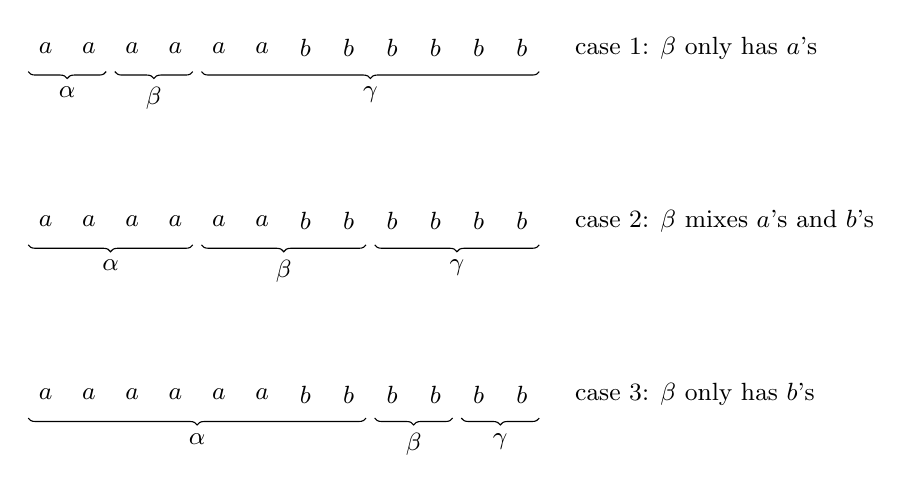
\begin{tikzpicture}[x=0.55cm, y=0.5cm, font=\small]
  \foreach \i in {1,...,6} { \node at (\i,0) {$a$}; }
  \foreach \i in {7,...,12} { \node at (\i,0) {$b$}; }
  \draw[decorate, decoration={brace, mirror}] (0.6,-0.6) -- (2.4,-0.6) node[midway, below=2pt] {$\alpha$};
  \draw[decorate, decoration={brace, mirror}] (2.6,-0.6) -- (4.4,-0.6) node[midway, below=2pt] {$\beta$};
  \draw[decorate, decoration={brace, mirror}] (4.6,-0.6) -- (12.4,-0.6) node[midway, below=2pt] {$\gamma$};
  \node[anchor=west] at (13,0) {case 1: $\beta$ only has $a$'s};

  \begin{scope}[yshift=-2.2cm]
  \foreach \i in {1,...,6} { \node at (\i,0) {$a$}; }
  \foreach \i in {7,...,12} { \node at (\i,0) {$b$}; }
  \draw[decorate, decoration={brace, mirror}] (0.6,-0.6) -- (4.4,-0.6) node[midway, below=2pt] {$\alpha$};
  \draw[decorate, decoration={brace, mirror}] (4.6,-0.6) -- (8.4,-0.6) node[midway, below=2pt] {$\beta$};
  \draw[decorate, decoration={brace, mirror}] (8.6,-0.6) -- (12.4,-0.6) node[midway, below=2pt] {$\gamma$};
  \node[anchor=west] at (13,0) {case 2: $\beta$ mixes $a$'s and $b$'s};
  \end{scope}

  \begin{scope}[yshift=-4.4cm]
  \foreach \i in {1,...,6} { \node at (\i,0) {$a$}; }
  \foreach \i in {7,...,12} { \node at (\i,0) {$b$}; }
  \draw[decorate, decoration={brace, mirror}] (0.6,-0.6) -- (8.4,-0.6) node[midway, below=2pt] {$\alpha$};
  \draw[decorate, decoration={brace, mirror}] (8.6,-0.6) -- (10.4,-0.6) node[midway, below=2pt] {$\beta$};
  \draw[decorate, decoration={brace, mirror}] (10.6,-0.6) -- (12.4,-0.6) node[midway, below=2pt] {$\gamma$};
  \node[anchor=west] at (13,0) {case 3: $\beta$ only has $b$'s};
  \end{scope}
\end{tikzpicture}
\caption{The three ways to split $a^k b^k$ (here $k = 6$). Cases 2 and 3 have
$|\alpha\beta| > k$, so only case 1 is allowed.}
\label{fig:pumping}
\end{figure}

So $\alpha = a^s$, $\beta = a^t$ and $\gamma = a^x b^k$, with $s + t + x = k$ and
$t > 0$. The lemma says that $\alpha\beta^n\gamma = a^{s + nt + x} b^k \in L$ for
every $n$, which requires $s + nt + x = k$. Take $n = 0$:
\begin{align*}
s + 0 \cdot t + x &= k && \langle n = 0 \rangle \\
s + x &= k && \langle \text{arithmetic} \rangle \\
s + x &= s + t + x && \langle \text{hypothesis } s + t + x = k \rangle
\end{align*}
which only holds if $t = 0$. But $t > 0$. This contradiction shows that the
assumption was false, and $L$ is not regular.

A consequence of the example is that regular languages cannot count: an
automaton with finitely many states cannot remember how many $a$'s it has
read in order to compare with the $b$'s. Languages that need this, such as
balanced parentheses, need a larger class: the context-free languages of
Section~\ref{sec:cfl}.

\subsection{Regular expressions in practice}

This subsection goes beyond the slides.

\paragraph{Thompson's construction.} The proof that every regular expression
has an automaton can be turned into an algorithm. Thompson's construction
builds an NFA fragment with one initial and one final state for each case of
the definition and glues the fragments with $\lambda$-transitions, the same way
as the union, concatenation and star of Section~\ref{sec:automata}.
Figure~\ref{fig:thompson} shows the result for $a^*b$. A person would draw
two states; the construction is meant for a program, and minimizing the
automaton is a separate step.

\begin{figure}[h]
\centering
\begin{tikzpicture}[node distance=2cm, auto]
  \node[state, initial] (s0) {$s_0$};
  \node[state, right=of s0] (s1) {$s_1$};
  \node[state, right=of s1] (s2) {$s_2$};
  \node[state, right=of s2] (s3) {$s_3$};
  \node[state, accepting, right=of s3] (s4) {$s_4$};
  \path[->]
    (s0) edge node {$\lambda$} (s1)
    (s1) edge[loop above] node {$a$} ()
    (s1) edge node {$\lambda$} (s2)
    (s2) edge node {$b$} (s3)
    (s0) edge[bend right=35] node[swap] {$\lambda$} (s2)
    (s3) edge node {$\lambda$} (s4);
\end{tikzpicture}
\caption{An NFA built by Thompson's construction for $a^*b$.}
\label{fig:thompson}
\end{figure}

\paragraph{Regular expression libraries.} The syntax of \texttt{grep}, Python's
\texttt{re} or Java's \texttt{Pattern} has the same three operators plus
abbreviations: character classes such as \texttt{[a-z]} are unions,
\texttt{\{2,\}} is a bounded repetition and \texttt{\textbackslash{}d} is
\texttt{[0-9]}.
\codelines{Python}{python/practical_regex.py}{3}{5}
Some features of these libraries are not regular. A backreference such as
\texttt{(\textbackslash{}w+) \textbackslash{}1} matches a word repeated twice,
and to do that for words of any length an automaton would need to remember
the whole first word. The test file shows it matching \texttt{is is}. Engines
that support backreferences search by backtracking instead of simulating an
automaton, and on some inputs they take exponential time, which a DFA never
does.

\paragraph{Forward pointer.} The tokens of a programming language (numbers,
identifiers, keywords, operators) are regular languages, and a lexer is a
finite automaton that recognizes all of them at once. The next block builds
one.

\subsection{Exercises}

\begin{exercise}
Which of the following match $(A..G)^+(\flat \mid \sharp)?$\,:
$A\flat$, $C\sharp$, $ABK\flat$, $A\flat B$, $GFE$?
\end{exercise}

\paragraph{Solution.} $A\flat$, $C\sharp$ and $GFE$ match. $ABK\flat$ does not,
because $K$ is not in $A..G$. $A\flat B$ does not either: the accidental can
only appear once, at the end.

\begin{exercise}
Write regular expressions for: (a) ``hello world'' in English; (b) a consonant
between every two pairs of vowels; (c) the words over $\{0,1\}$ that contain
$00$; (d) the words over $\{a,b\}$ where two $a$'s never come together;
(e) the words over $\{0,1\}$ that start with 0 and have odd length or start
with 1 and have even length.
\end{exercise}

\paragraph{Solution.}
(a) The expression \texttt{hello world} itself: a fixed word is a
concatenation of symbols.
(b) With $V = (a \mid e \mid i \mid o \mid u)$ and $C = (b \mid c \mid d \mid \dots \mid z)$
without the vowels, the lecture's answer is $(VVCVV)^*$. Two blocks next to
each other give $VVCVVVVCVV$, with four vowels together; if the intended
words are pairs of vowels separated by one consonant, the expression is
$\lambda \mid VV(CVV)^*$.
(c) $(0 \mid 1)^*00(0 \mid 1)^*$.
(d) $a(b \mid ba)^* \mid (b \mid ba)^*$: every $a$ after the first symbol is
preceded by a $b$.
(e) $0((0 \mid 1)(0 \mid 1))^* \mid 1(0 \mid 1)((0 \mid 1)(0 \mid 1))^*$. The answer on
the slide ends with $1(0 \mid 1)^*$, which accepts the words that start with
1 of any length, for example $1$ itself.

\begin{exercise}
Write a regular expression that checks that an e-mail address belongs to the
domain \texttt{uniandes.edu.co}. Then write one for any e-mail address.
\end{exercise}

\paragraph{Solution.} The slides write character sets with braces; in the
usual syntax of regular expression libraries:
\codelines{Rascal}{rascal/src/Regular.rsc}{44}{45}
The braces on the slides mean repetition, as in EBNF, so the slide's
version also accepts an address with nothing before the \texttt{@}; the
\texttt{+} above requires at least one character. The dots of the domain are
escaped because an unescaped dot means any character.

\begin{exercise}
Consider the grammar $s ::= (bc)^*t$, $b ::= m^+ \mid pbt$, $c ::= b \mid e^+$.
What are the nonterminals, the terminals and the recursive rules? Is the
grammar regular?
\end{exercise}

\paragraph{Solution.} The nonterminals are the symbols that have rules: $s$, $b$
and $c$. The terminals are $t$, $m$, $p$ and $e$. The symbols \texttt{|},
\texttt{*} and \texttt{+} belong to the notation, not to the grammar. The only
recursive rule is $b ::= pbt$. It has a nonterminal in the middle of its right
side, so the grammar is not regular, and indeed $b$ generates
$p^n m^+ t^n$, which needs to count.

\begin{exercise}
For each language over $\{0,1\}$, write a regular expression and an automaton:
(1) the number of 0s is divisible by 3; (2) even number of 0s; (3) the fifth
symbol from the right is 1; (4) each 0 is followed by at least one 1;
(5) $0^n 1^m$ with $n \ge 3$ and $m$ even; (6) at most two 0s; (7) start with 0
and have odd length or start with 1 and have even length; (8) any word except
$0$ and $1$; (9) words that do not end with $01$.
\end{exercise}

\paragraph{Solution.} Table~\ref{tab:nine} gives the expressions and
Figures~\ref{fig:nine-a}--\ref{fig:nine-c} the automata. All nine
expressions and automata are in \texttt{Regular.rsc}, and the tests compare
them with a direct definition of each language on every word of length up
to 9.

\begin{table}[h]
\centering
\small
\begin{tabular}{l l l}
  \toprule
  & Language & Regular expression \\
  \midrule
  1 & 0s divisible by 3         & $(1 \mid 01^*01^*0)^*$ \\
  2 & even number of 0s         & $(1 \mid 01^*0)^*$ \\
  3 & fifth from the right is 1 & $(0 \mid 1)^*1(0 \mid 1)(0 \mid 1)(0 \mid 1)(0 \mid 1)$ \\
  4 & each 0 followed by a 1    & $(0?1)^*$ \\
  5 & $0^n1^m$, $n \ge 3$, $m$ even & $000^*0(11)^*$ \\
  6 & at most two 0s            & $1^*0?1^*0?1^*$ \\
  7 & odd with 0, even with 1   & $(0 \mid 1(0 \mid 1))((0 \mid 1)(0 \mid 1))^*$ \\
  8 & not $0$, not $1$          & $\lambda \mid (0 \mid 1)(0 \mid 1)(0 \mid 1)^*$ \\
  9 & not ending in $01$        & $\lambda \mid 0 \mid 1 \mid (0 \mid 1)^*(0 \mid 1(0 \mid 1))$ \\
  \bottomrule
\end{tabular}
\caption{Regular expressions for the nine languages.}
\label{tab:nine}
\end{table}

A few notes. In (1) each group of three 0s may have 1s between them, and the
outer star allows 1s anywhere else. In (5) the expression $000^*0$ is the
lecture's way of writing at least three 0s ($00$, then $0^*$, then $0$). The
slide's expressions for (8) and (9) leave out $\lambda$, which belongs to both
languages: the empty word is neither $0$ nor $1$, and it does not end with
$01$. The slide's automaton for (9) has the transitions
$0 \xrightarrow{1} 0$, $0 \xrightarrow{0} 0$, $0 \xrightarrow{0} 1$,
$0 \xrightarrow{1} 2$, $2 \xrightarrow{1} 3$ and final states $\{1, 2, 3\}$. It
accepts $01$: from 0 it reads 0 and stays, then reads 1 and goes to the final
state 2. The automaton of Figure~\ref{fig:nine-c} remembers the last two
symbols instead.

\begin{figure}[h]
\centering
\begin{tikzpicture}[node distance=1.6cm, auto]
  \node at (-0.9,1) {(1)};
  \node[state, initial, accepting] (a0) {0};
  \node[state, right=of a0] (a1) {1};
  \node[state, below right=1cm and 0.5cm of a0] (a2) {2};
  \path[->]
    (a0) edge node {0} (a1)
    (a1) edge node {0} (a2)
    (a2) edge node {0} (a0)
    (a0) edge[loop above] node {1} ()
    (a1) edge[loop above] node {1} ()
    (a2) edge[loop right] node {1} ();
\end{tikzpicture}
\hspace{0.8cm}
\begin{tikzpicture}[node distance=1.6cm, auto]
  \node at (-0.9,1) {(2)};
  \node[state, initial, accepting] (b0) {0};
  \node[state, right=of b0] (b1) {1};
  \path[->]
    (b0) edge[bend left] node {0} (b1)
    (b1) edge[bend left] node {0} (b0)
    (b0) edge[loop above] node {1} ()
    (b1) edge[loop above] node {1} ();
\end{tikzpicture}
\hspace{0.8cm}
\begin{tikzpicture}[node distance=1.6cm, auto]
  \node at (-0.9,1) {(4)};
  \node[state, initial, accepting] (d1) {1};
  \node[state, right=of d1] (d0) {0};
  \path[->]
    (d1) edge[loop above] node {1} ()
    (d1) edge[bend left] node {0} (d0)
    (d0) edge[bend left] node {1} (d1);
\end{tikzpicture}

\vspace{0.6cm}
\begin{tikzpicture}[node distance=1.3cm, auto]
  \node at (-0.9,0.9) {(3)};
  \node[state, initial] (c0) {0};
  \node[state, right=of c0] (c1) {1};
  \node[state, right=of c1] (c2) {2};
  \node[state, right=of c2] (c3) {3};
  \node[state, right=of c3] (c4) {4};
  \node[state, accepting, right=of c4] (c5) {5};
  \path[->]
    (c0) edge[loop above] node {0, 1} ()
    (c0) edge node {1} (c1)
    (c1) edge node {0, 1} (c2)
    (c2) edge node {0, 1} (c3)
    (c3) edge node {0, 1} (c4)
    (c4) edge node {0, 1} (c5);
\end{tikzpicture}
\caption{Automata for languages (1), (2), (4) and (3). The automaton for (3)
is nondeterministic: in state 0 it guesses that the current 1 is the fifth
symbol from the end. In (4) a 0 with no 1 after it gets stuck.}
\label{fig:nine-a}
\end{figure}

\begin{figure}[h]
\centering
\begin{tikzpicture}[node distance=1.5cm, auto]
  \node at (-0.9,1) {(5)};
  \node[state, initial] (e0) {0};
  \node[state, right=of e0] (e1) {1};
  \node[state, right=of e1] (e2) {2};
  \node[state, accepting, right=of e2] (e3) {3};
  \node[state, right=of e3] (e4) {4};
  \path[->]
    (e0) edge node {0} (e1)
    (e1) edge node {0} (e2)
    (e2) edge[loop above] node {0} ()
    (e2) edge node {0} (e3)
    (e3) edge[bend left] node {1} (e4)
    (e4) edge[bend left] node {1} (e3);
\end{tikzpicture}
\hspace{0.8cm}
\begin{tikzpicture}[node distance=1.5cm, auto]
  \node at (-0.9,1) {(6)};
  \node[state, initial, accepting] (f0) {0};
  \node[state, accepting, right=of f0] (f1) {1};
  \node[state, accepting, right=of f1] (f2) {2};
  \path[->]
    (f0) edge node {0} (f1)
    (f1) edge node {0} (f2)
    (f0) edge[loop above] node {1} ()
    (f1) edge[loop above] node {1} ()
    (f2) edge[loop above] node {1} ();
\end{tikzpicture}
\caption{Automata for languages (5) and (6). In (5) the loop on state 2 makes
the automaton nondeterministic; in (6) a third 0 gets stuck.}
\label{fig:nine-b}
\end{figure}

\begin{figure}[h]
\centering
\begin{tikzpicture}[node distance=1.6cm, auto]
  \node at (-0.9,1.2) {(7)};
  \node[state, initial] (g0) {0};
  \node[state, above right=0.8cm and 1.4cm of g0] (g1) {1};
  \node[state, accepting, right=of g1] (g3) {3};
  \node[state, accepting, below right=0.8cm and 1.4cm of g0] (g2) {2};
  \node[state, right=of g2] (g4) {4};
  \path[->]
    (g0) edge node {1} (g1)
    (g0) edge node[swap] {0} (g2)
    (g1) edge[bend left] node {0, 1} (g3)
    (g3) edge[bend left] node {0, 1} (g1)
    (g2) edge[bend left] node {0, 1} (g4)
    (g4) edge[bend left] node {0, 1} (g2);
\end{tikzpicture}
\hspace{0.6cm}
\begin{tikzpicture}[node distance=1.5cm, auto]
  \node at (-0.9,1) {(8)};
  \node[state, initial, accepting] (h0) {0};
  \node[state, right=of h0] (h1) {1};
  \node[state, accepting, right=of h1] (h3) {3};
  \path[->]
    (h0) edge node {0, 1} (h1)
    (h1) edge node {0, 1} (h3)
    (h3) edge[loop above] node {0, 1} ();
\end{tikzpicture}

\vspace{0.6cm}
\begin{tikzpicture}[node distance=2cm, auto]
  \node at (-0.9,1) {(9)};
  \node[state, initial, accepting] (s) {$s$};
  \node[state, accepting, right=of s] (z) {$z$};
  \node[state, right=of z] (zo) {$zo$};
  \path[->]
    (s) edge[loop above] node {1} ()
    (s) edge node {0} (z)
    (z) edge[loop above] node {0} ()
    (z) edge[bend left] node {1} (zo)
    (zo) edge[bend left] node {0} (z)
    (zo) edge[bend left=45] node {1} (s);
\end{tikzpicture}
\caption{Automata for languages (7), (8) and (9). In (7) the states 1 and 3
count parity after a first 1, and 2 and 4 after a first 0. In (9) the state
$z$ means ``the last symbol is 0'' and $zo$ means ``the last two symbols are
01''.}
\label{fig:nine-c}
\end{figure}

\begin{exercise}
Is \texttt{12-11-2025} a word of the date language? And \texttt{02/31/2000}? Change the
grammar so that \texttt{Dash} also accepts four-digit years.
\end{exercise}

\paragraph{Solution.} \texttt{12-11-2025} is not: \texttt{Dash} ends after two year
digits. \texttt{02/31/2000} is, even though the date does not exist. Replacing the
end of \texttt{Dash} with \texttt{(Year Year | Year1 Year Year Year)} accepts
both two- and four-digit years.

\begin{exercise}
Use the pumping lemma to show that $\{0^n 1 0^n \mid n \ge 0\}$ is not regular.
\end{exercise}

\paragraph{Solution.} Given $k$, take $\omega = 0^k 1 0^k$. Since
$|\alpha\beta| \le k$, $\beta = 0^t$ with $t > 0$ lies in the first block of 0s.
With $n = 0$ the word becomes $0^{k-t} 1 0^k$, which has fewer 0s before the
1 than after it, so it is not in the language.
